%%
%% IMPORTANT NOTICE:
%% A paper about using geohash to control epidemic
%% Use covid-19 as example
%% Youwei Huang
%% IICT, CAS
\documentclass[sigplan,screen]{acmart}
\usepackage{subfigure}
\AtBeginDocument{%
  \providecommand\BibTeX{{%
    \normalfont B\kern-0.5em{\scshape i\kern-0.25em b}\kern-0.8em\TeX}}}
\setcopyright{acmcopyright}
\copyrightyear{2018}
\acmYear{2018}
\acmDOI{10.1145/1122445.1122456}
\acmConference[Woodstock '18]{Woodstock '18: ACM Symposium on Neural
  Gaze Detection}{June 03--05, 2018}{Woodstock, NY}
\acmBooktitle{Woodstock '18: ACM Symposium on Neural Gaze Detection,
  June 03--05, 2018, Woodstock, NY}
\acmPrice{15.00}
\acmISBN{978\-1\-4503-XXXX-X/18/06}
\begin{document}
\title{Epidemics Prevention and Control Based On GeoHash}
\author{Youwei Huang (Project Manager)}
\email{huangyw@iict.ac.cn}
\affiliation{%
	\institution{Institute of Intelligent Computing Technology, Chinese Academy of Sciences}
	\city{Suzhou}
	\state{Jiangsu}
	\country{China}
	\postcode{215000}
}
\author{Feng Lu (Algorithm Engineer)}
\email{lufeng20g@ict.ac.cn}
\affiliation{%
	\institution{Institute of Computing Technology, Chinese Academy of Sciences}
	\city{Beijing}
	\country{China}}
%% Abstract
\begin{abstract}
	COVID-19 (Coronavirus Disease 2019) which is a contagious disease caused by SARS-CoV-2\cite{hu2020characteristics} was first detected in Dec. 2019.
	Until today 2021, this virus is still spreading around the world.
	Before the vaccine is widely vaccinated or the invention of specific medication, many measures have been taken by people to prevent the spread of the epidemic.
	In a special period, we have to quarantine the high-risk groups and lock down seriously infected regions.
	Here we propose a kind of dynamic block division technology based on \textbf{GeoHash} used to monitor, screen and control the epidemic areas.
	\textbf{GeoHash} is a public domain geocode system invented in 2008 by Gustavo Niemeyer\cite{niemeyer2008geohash}.
	We divide a map into several blocks and use \textbf{GeoHash} to encode the information of each block.
	Through the \textbf{GIS}, \textbf{GeoHash} can be easily decoded to original visual blocks on the digital map.
	A map generated by \textbf{GIS} is used for epidemic prevention and control, so it is named \textbf{``Epidemic Map''}.
	Each block on such \textbf{Epidemic Map} contains the safety information and other important characteristics which are concerned by medical work.
	These dynamic blocks on the map can be scaled and represented as various regular geometric shapes.
	The vital information and the results of quantitative analysis of the data on each block support for decision-making, measures formulation, and effectiveness assessment of COVID-19 prevention and control.
	Such a kind of geographic information system can be used not only for preventing and controlling COVID-19 pandemic, but also be applicative in instances of other epidemic diseases.
\end{abstract}
\keywords{GeoHash, COVID-19, GIS, big data, epidemic prevention and control}
\begin{teaserfigure}
	\centering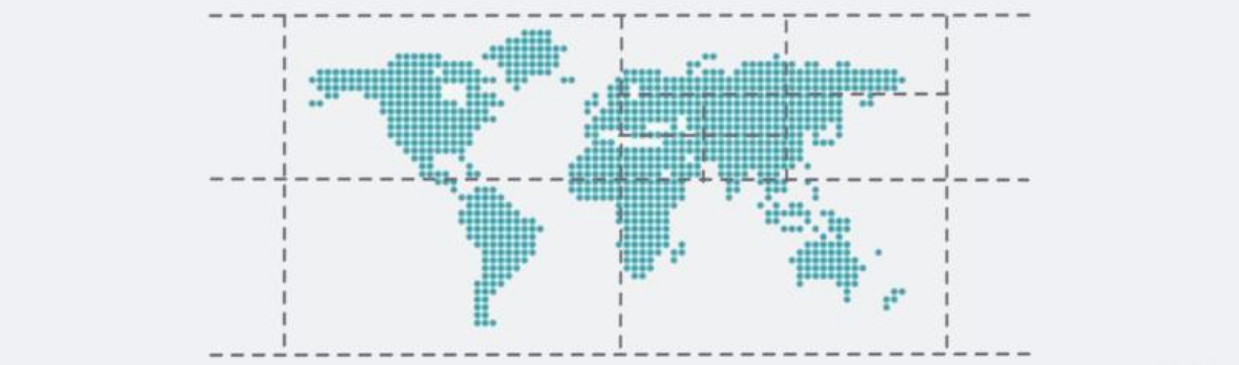
\includegraphics[height=50mm]{logo.png}
	\caption{GeoHash technology for geographic grid division}
	\Description{In 2008, Gustavo Niemeyer invented GeoHash which encoded a geographic location into a short string}
	\label{fig:teaser}
\end{teaserfigure}
%%
%% This command processes the author and affiliation and title
%% information and builds the first part of the formatted document.
\maketitle
\section{Introduction}
During the COVID-19 pandemic, many cities over the world were forced to lock down.
Wuhan City and the major cities in Hubei, China were put under lockdown on the 23rd and 24th of January, respectively\cite{lau2020positive}.
Lockdown meant the whole region was quarantined and cut off physical contact with the outside world.
The citizens were forbidden to leave their city or even their home.
The national medical team carried out centralized medical observation and treatment in quarantined cities.
Research shows, COVID-19 spread became weaker following lockdown\cite{lau2020positive}.
However the lockdown of a city can cause huge economic losses.
The lockdown of Some vital areas can cause irreparable losses, such as financial center, political center, and industrial dependent cities.
Another issue is how our people can make sure whether the area they are in or the area they are going to is safe.
The current regional risk warning or lockdown is based on the administrative divisions as figure 2.
Cities, states or provinces all over the world have different sizes and irregular geographic borders.
There may be an outbreak in a city, but it does not mean that it spreads to all corners of the city.
On the contrary, there may be no epidemic in the center of neighboring cities, but there may already be a huge risk at the border with these surrounding cities.
Figure 2 is a map that shows the initial locked down cities in Wuhan province, a white block surrounded by red blocks is dangerous, even if it is not locked down.
\begin{figure}[htb]
	\centering
	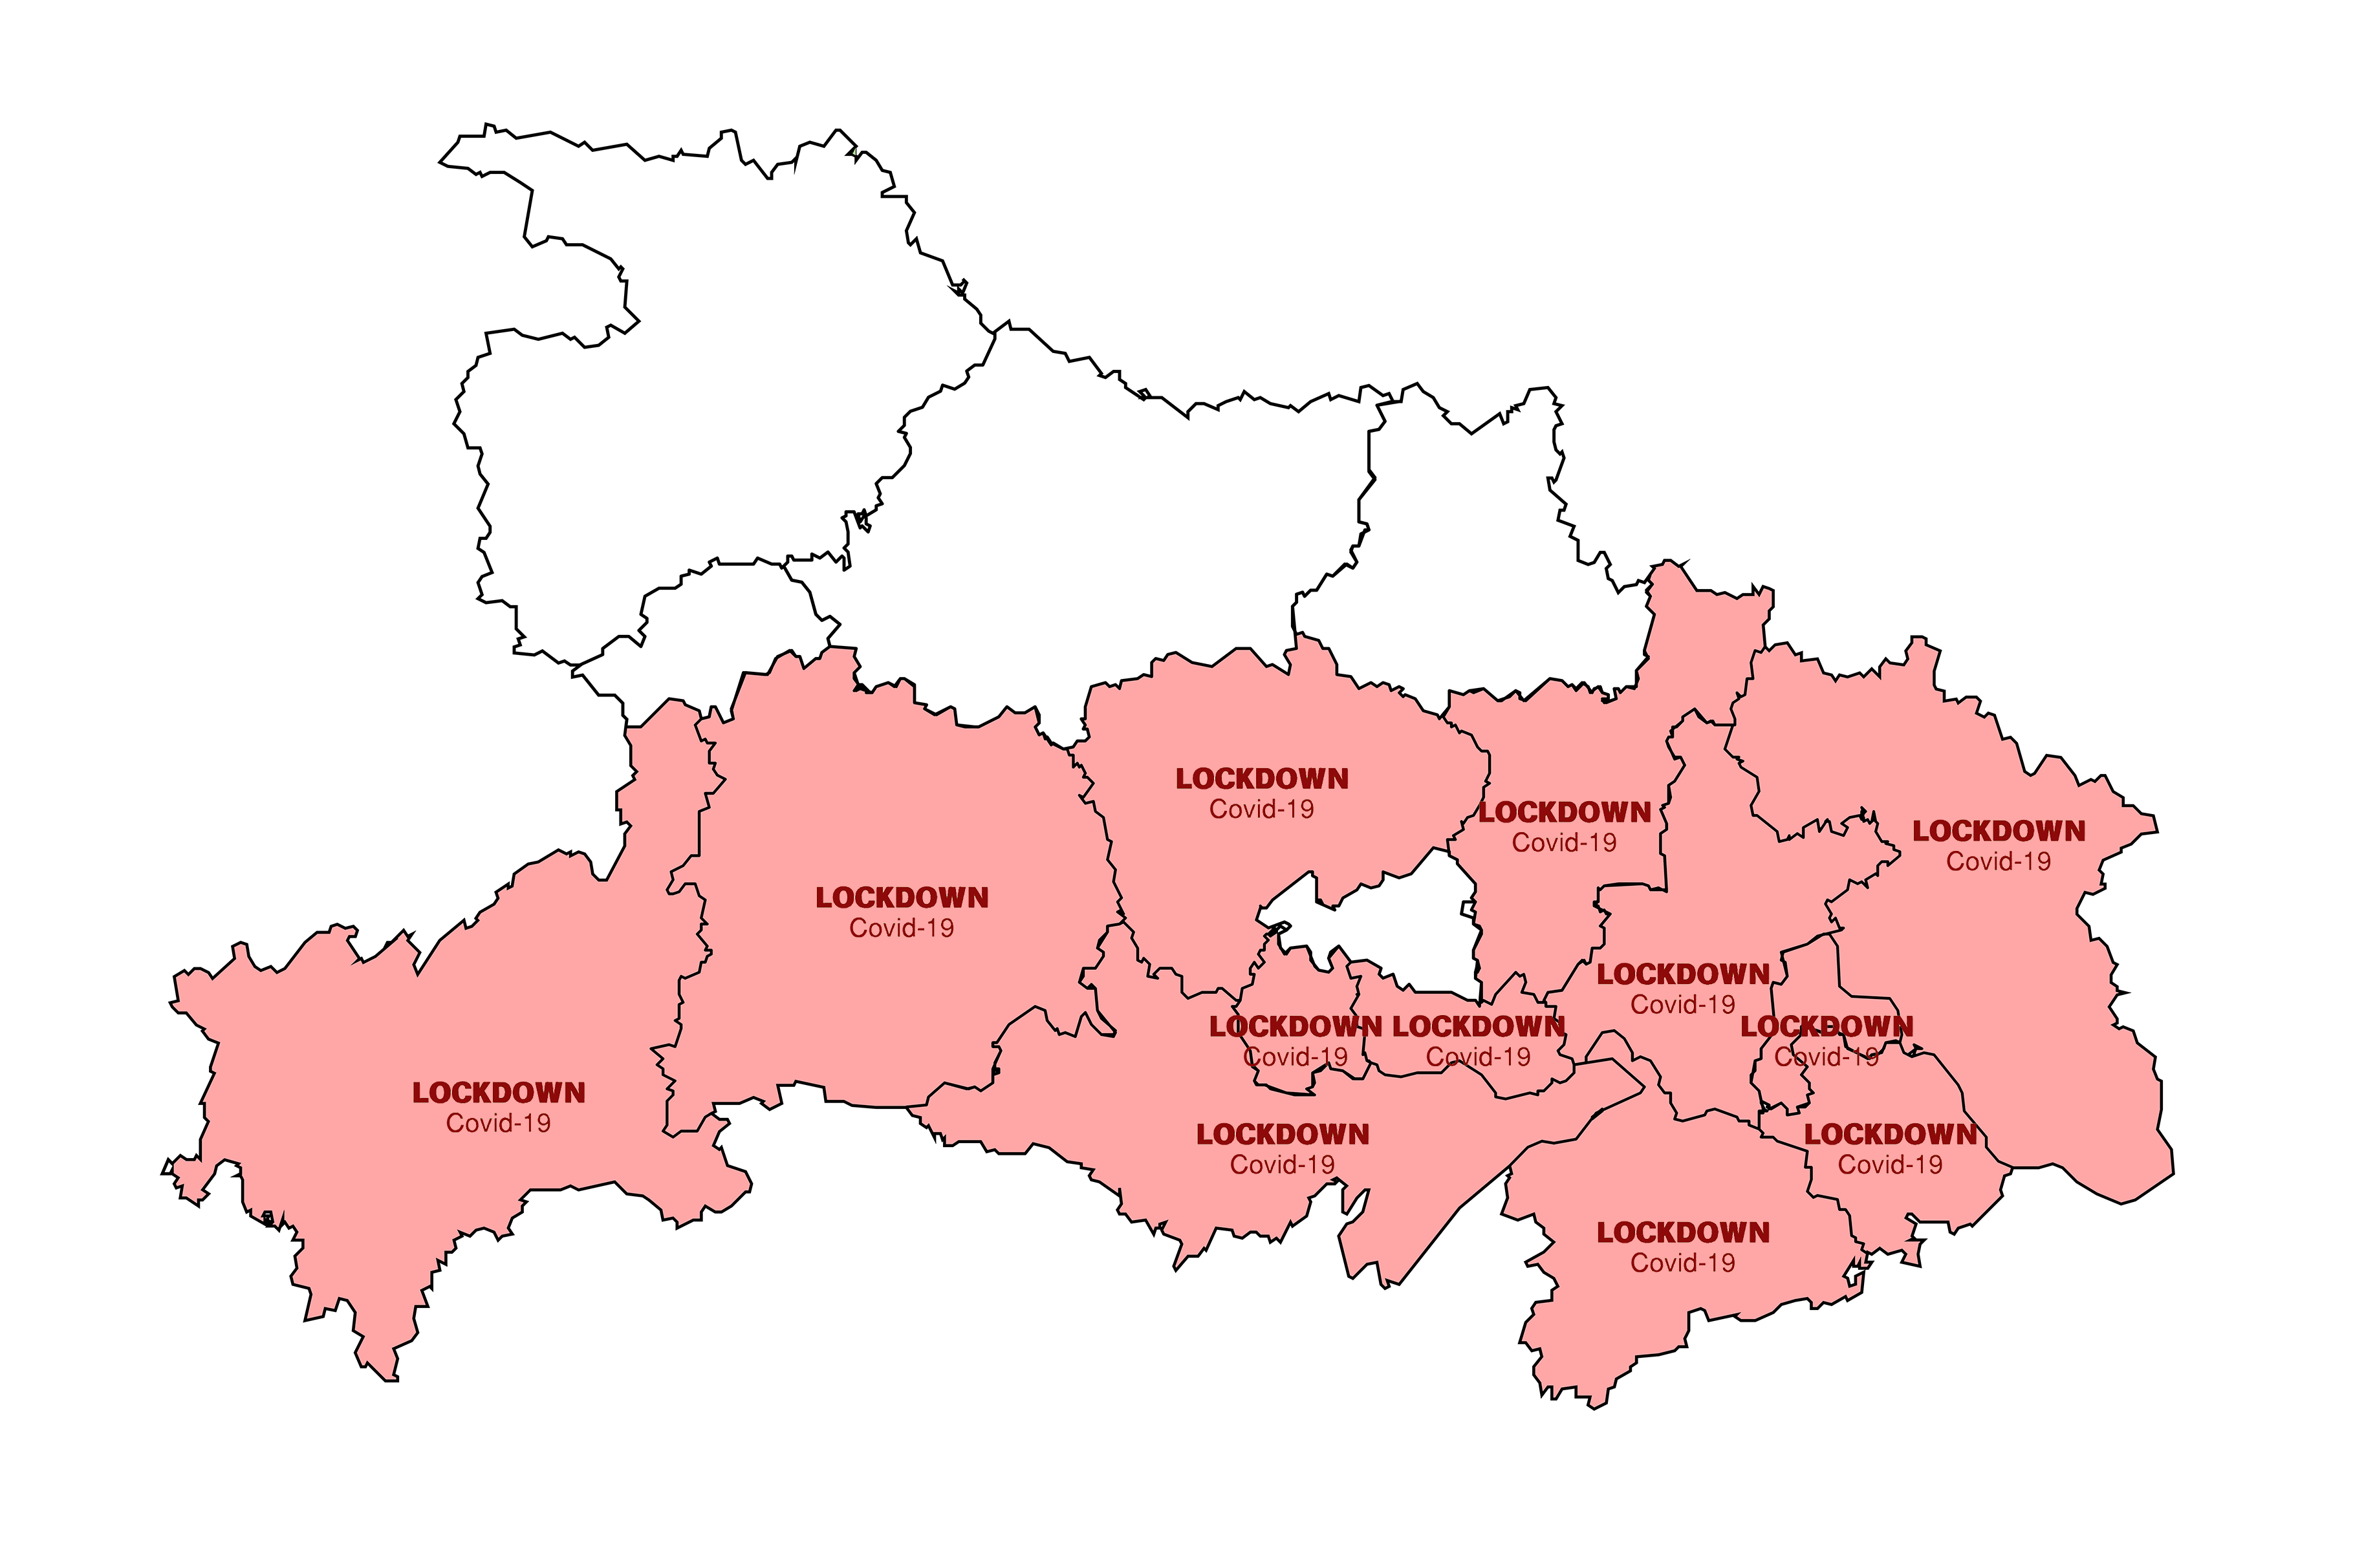
\includegraphics[width=\linewidth]{hubei.png}
	\caption{Map of locked down administrative divisions of Hubei. [Public domain], via Wikipedia. (\url{https://en.wikipedia.org/wiki/COVID-19_lockdown_in_Hubei}).}
	\Description{Locked down cities in Hubei province, white blocks are unlocked and red blocks are locked}
\end{figure}
\\
We summarize the main weaknesses by using the current dividing measures to mark area safety level:
\begin{enumerate}
	\item The border of a city is irregular and the transmission of virus doesn't follow the administrative division, so the prevention and lockdown can be not accurate.
	\item The administrative size of a city is fixed, but the disease is spreadable, so the region of lockdown can not be expanded flexibly.
	\item Due to regional differences, the information released in each region is not complete and not uniform.
	\item The news released by the local government can be lagging and users cannot get it in real time.
\end{enumerate}
Based on above points of view, it is not the best way to observe and control the epidemic area through the administrative division.
For infectious diseases, we have abandoned the common administrative methods. And we have adopted a technology based on GIS (Geographic Information System)\cite{clarke1986advances}. \textbf{GeoHash} is used to divide the map into several geometric blocks. The 2-dimensional geometric blocks on the map are encoded by GeoHash, they are reduced to 1-dimension and stored as string in any databases. These blocks are presented as regular geometry, but can be scaled according to the needs of different observation scope.
\\
Meanwhile, we do this technology is because it has the following advantages when controlling epidemic situation:
\begin{enumerate}
	\item The blocks divided by GeoHash are regular geometry, and the shape can be customized by observer.
	\item The blocks are generated dynamically and they are scalable according to the scope of infection.
	\item By combining with GIS, information about the epidemic situation can be encoded in GeoHash or directly saved.
	\item Block data can be easily quantified, as example of generating safety index.
	\item When such a GIS is released to the Internet, users get epidemic information in real time.
\end{enumerate}
In the practical and experimental scenarios, we use mobile application and web technology to develop such a particular GIS for medical prevention and treatment as Figure 3. It works for medical workers as a visual auxiliary tool and share the results of epidemic data analysis. The \textbf{ASI} in Figure 3 is a value of ``Area Safety Index''. \textbf{ASI} represents the risk level of a region. The system contributes to enlighten and support decisions of governments, medical institutions, users, and other researchers who are doing the similar research with us.
\\
The core idea of this technology is dividing the earth to dynamic blocks. A block has the following characteristics:
\begin{enumerate}
	\item Blocks are regular geometry connected with each other. It can be understood as cellular grids.
	\item Blocks can be scaled on the map.
	\item Blocks are created only when they are meaningful.
	\item Scaling is limited, with the smallest and largest block size.
	\item Blocks scaling levels are discrete sizes, not continuous.
	\item A block stores structured data, which can be used for computing and analysing various attributes.
\end{enumerate}
The last item in the above list indicates that the purpose of dividing by blocks is to perform quantitative analysis related to the epidemic situation.
\\
We will also introduce other related work in controlling epidemic by using similar information technology and computer visualization technology.
Then we will focus on how we use \textbf{GeoHash} to divide blocks on the map, and explain the methods of quantifing epidemic data to provide area risk warning.
Finally, by using our GIS example, we will give our experimental and test results, and summarize the conclusion.
\begin{figure*}[hptb]
	\centering
	\subfigure[larger scale]{
		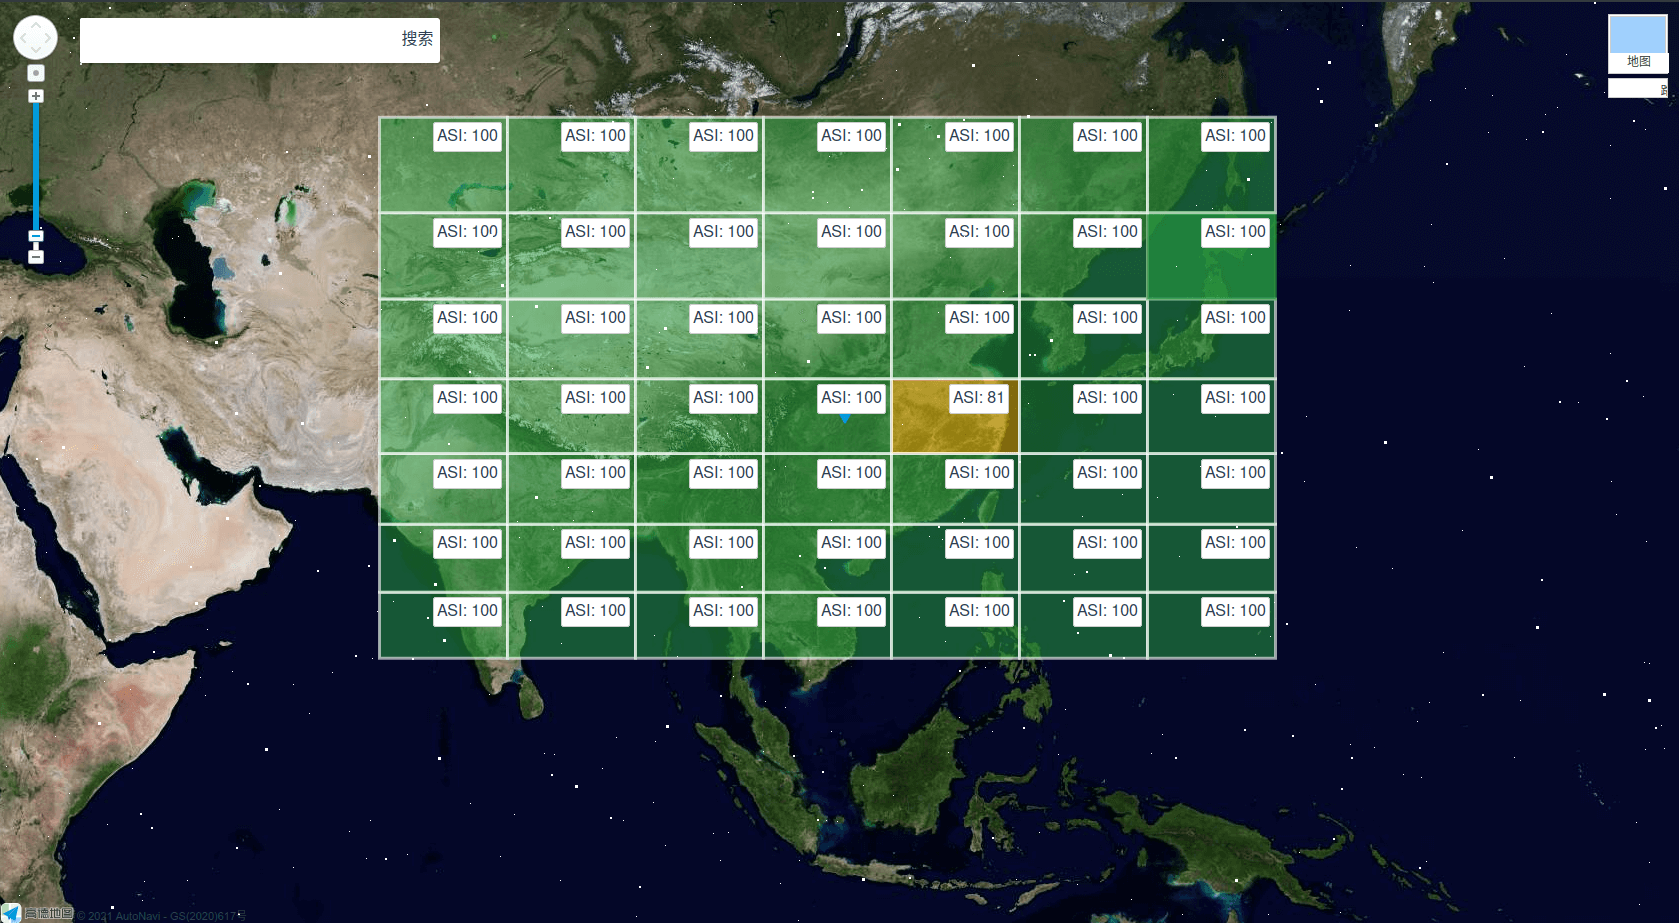
\includegraphics[width=\textwidth]{geogrids1.png}
	}
	\subfigure[smaller scale]{
		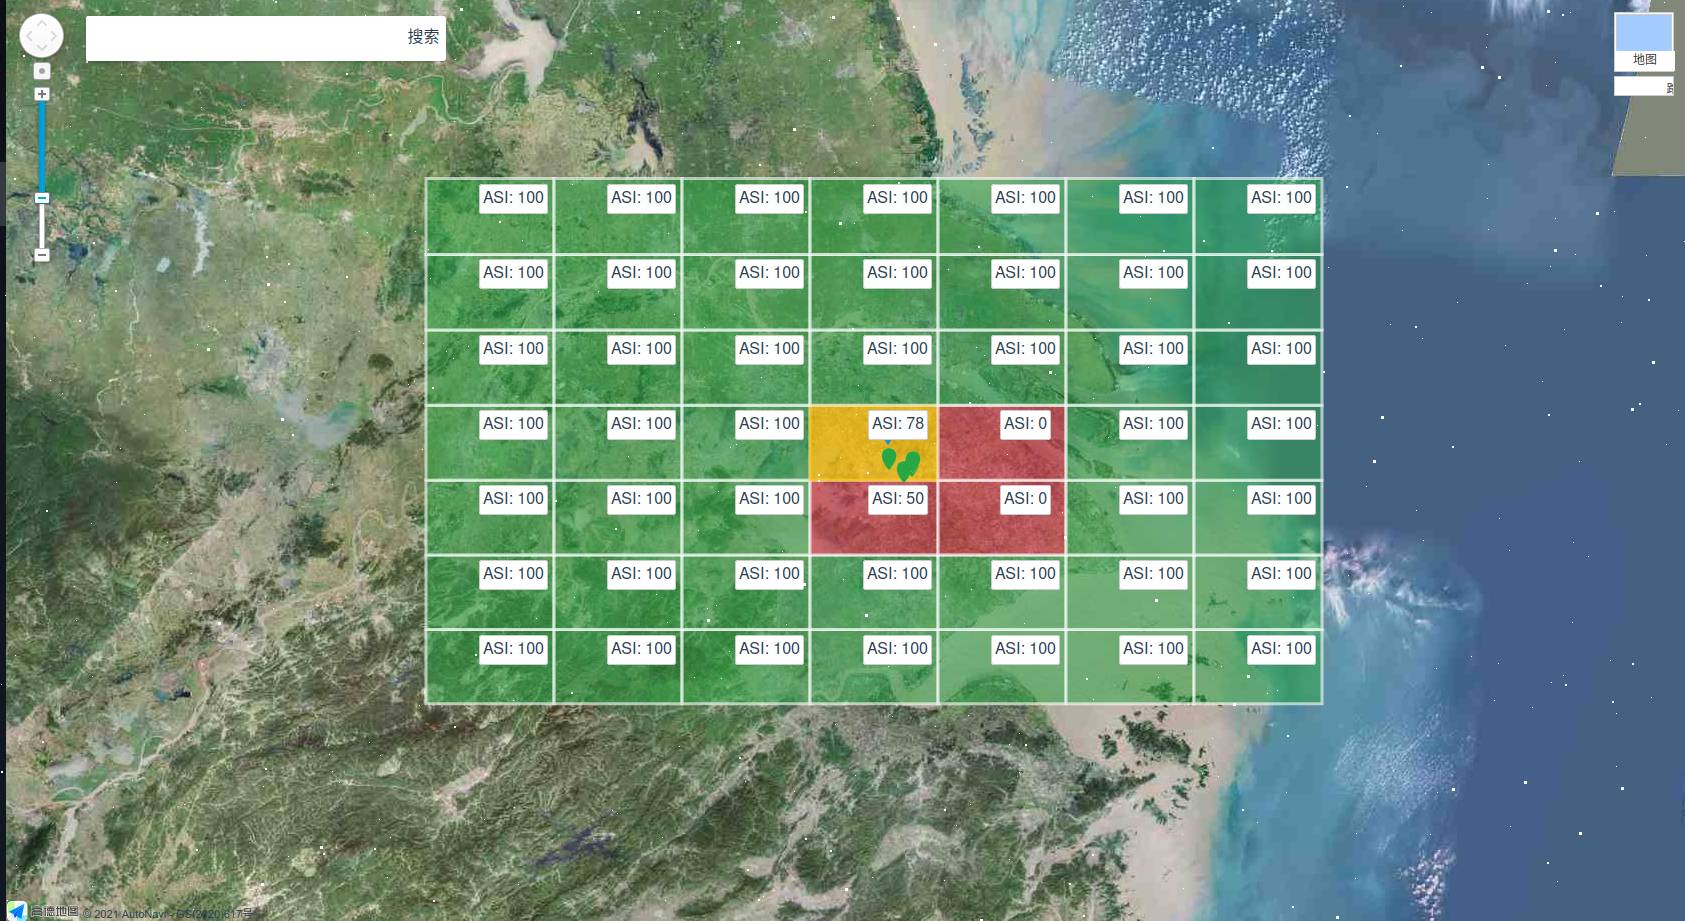
\includegraphics[width=\textwidth]{geogrids2.png}
	}
	\caption{Dynamic blocks with ASI in geographic information system}
\end{figure*}
\section{Related Work}
There are some mature cases of controlling and treating COVID-19 pandemic by using information technology and Internet data.
Many studies on COVID-19 have recently emerged, and various data science applications combating the pandemic have been reported recently\cite{latif2020leveraging}.
The main functions of these systems or softwares are listed as follows:\cite{jia2020big}
\begin{itemize}
	\item Tracking of people's movements.
	\item Early warning of high-risk areas.
	\item Screening of asymptomatic potential infections.
	\item Drug development.
	\item Information release and policy support.
\end{itemize}
\subsection{Data Visualization Analysis}
The computer can visualize all kinds of structured data and convey the visual information to users.
Visualization technology presents data to users by drawing charts and graphics, in which the data is represented by symbols, such as bar charts, line charts, pie charts, maps and etc\cite{jensen1992harvard}.
\\
Figure 4 shows the global COVID-19 epidemic situation in the form of map charts. The epidemic maps are updated by WHO (World Health Organization)\footnote{https://www.who.int} in real time, to display the number of cases around the world.
\begin{figure}[htb]
	\centering
	\subfigure[Choropleth Map]{
		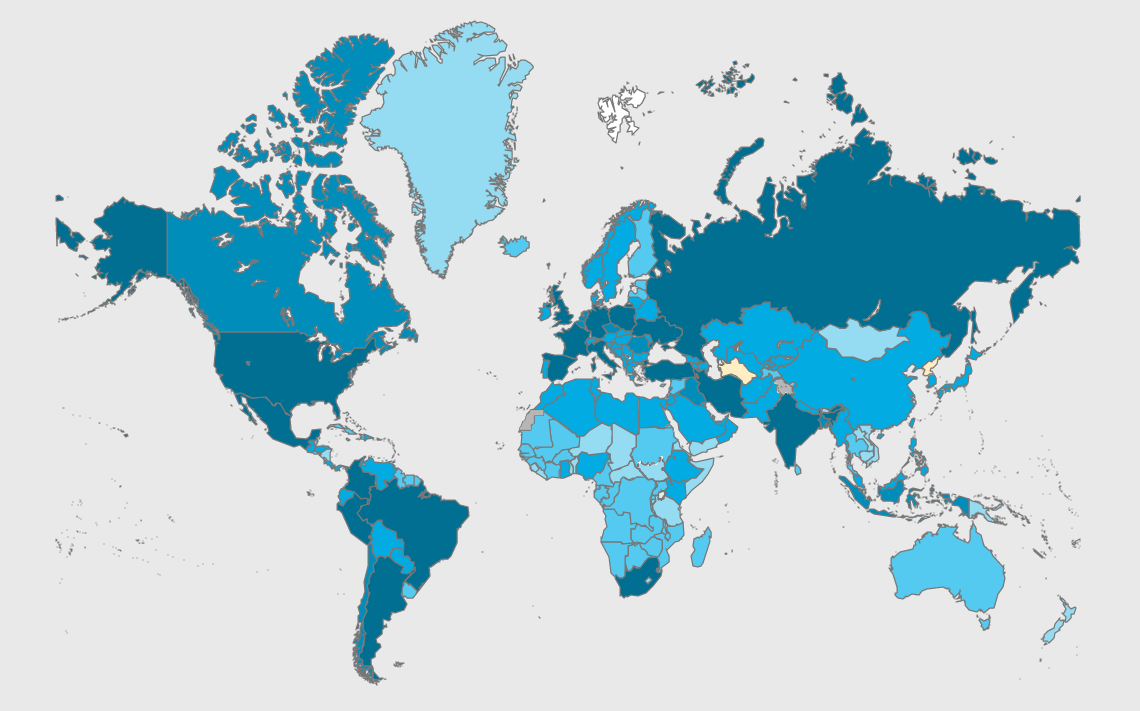
\includegraphics[width=\linewidth]{worldmap1.png}
	}
	\subfigure[Bubble Map]{
		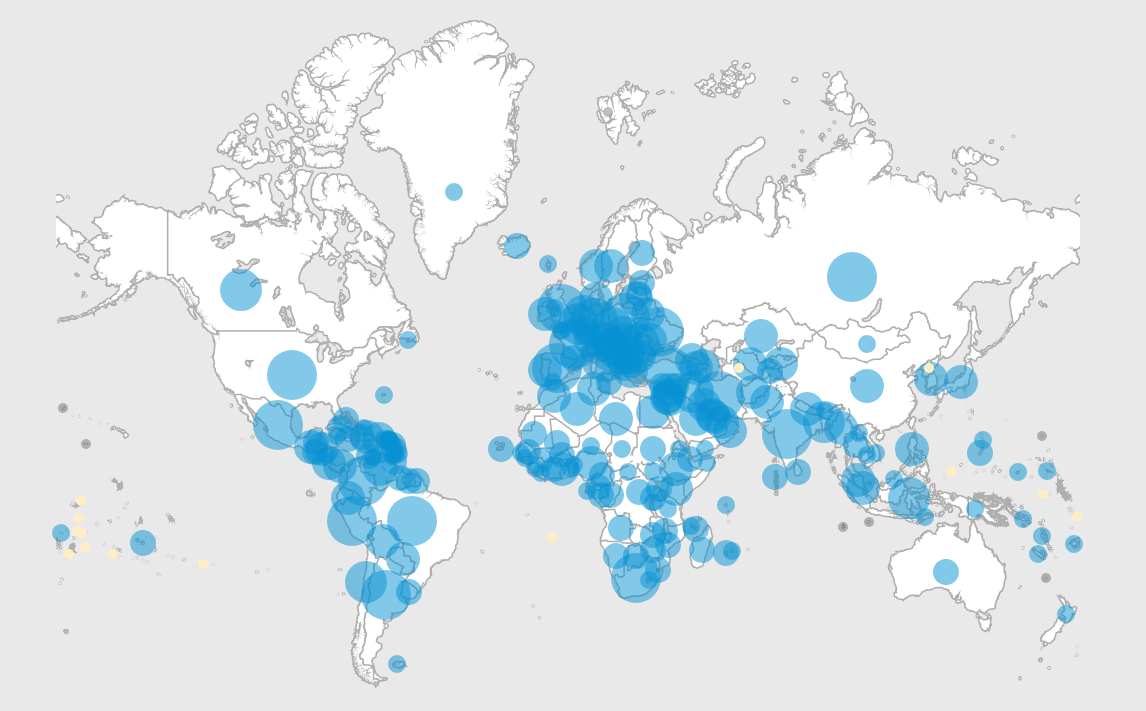
\includegraphics[width=\linewidth]{worldmap2.png}
	}
	\caption{WHO coronavirus disease dashboard. [Public domain], via WHO (\url{https://covid19.who.int})}
	\Description{The figures are captured from the official website of WHO, the web page uses a dashboard to show the COVID-19 situation over the world.}
\end{figure}
\\
Maps in Figure 4 uses two styles of presentation: choropleth and bubble.
One uses the depth of color to show the severity of the epidemic situation in each country, and another uses the bubble size to show the number of infections.
No matter what kind of map, its role is to help the local people easy to understand the severity of the epidemic, and prompt the local government to take actions to treat and control the epidemic situation.
These two figures (Figure 4) are similar to the previous Figure 2, except that Figure 2 only shows the data of one province.
Contents in these maps include like: confirmed cases, deaths, historical cases, added cases, and regional lockdown status.
Some disadvantages of such kind of maps are discussed in section 1: \textbf{Introduction}.
\\
The bar charts and line charts are aslo widely used in epidemic data analysis.
These graphs are mostly used to show the trend of epidemic situation and transmission cycle.
Figure 5 is an example that uses both bar chart and line chart to perform the trend of daily new cases from Jan. 2020 to Jan. 2021 in the US. The red line in this chart is the 7-day moving average curve.
We can also view other trends of different types of data, such as death trends, through the CDC\footnote{https://covid.cdc.gov/covid-data-tracker} official website.
\begin{figure}[htb]
	\centering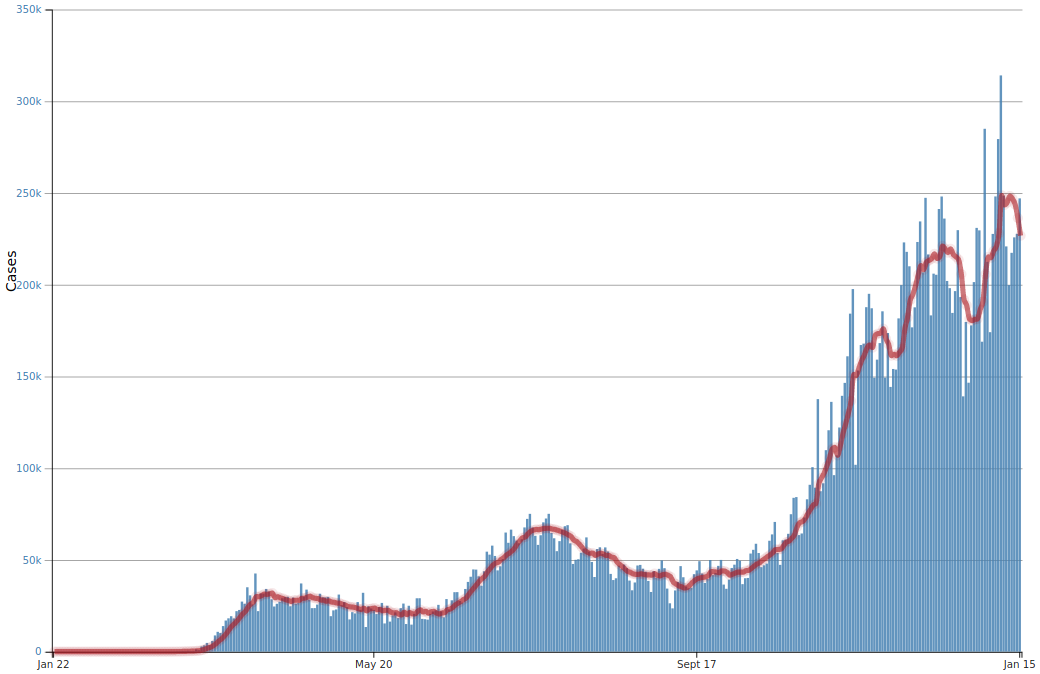
\includegraphics[width=\linewidth]{linebar-us-1-15.png}
	\caption{Daily trends in number of COVID-19 new cases in the US reported to CDC. [Public domain], via CDC (\url{https://covid.cdc.gov/covid-data-tracker/\#trends_dailytrendscases})}
	\Description{The figure is a screenshot from CDC official web page, it shows the daily new cases in the US by drawing a bar and line chart.}
\end{figure}
\\
The line charts and bar charts reflect historical epidemic data from time series, while map charts reflect epidemic data from spatial distribution.
In other related work survey, visual data analysis are used to study the relationship between population mobility and the epidemic spreading pattern.
During the early outbreak of coronavirus in Wuhan, China, the graphs in a research gave a conclusion that the number of confirmed cases in other provinces were directly proportional to the inflow of Wuhan population.
The research group also used the pattern derived from the data analysis to predict the number of infections.\cite{chen2020data}
\subsection{Geographic Information System}
The maps we described in the previous section are charts, the information carried by map charts is limited, unflexible and not real-time.
Although charts can provide visual perception, users need to analyze the graphs by themselves, but GIS can integrate analysis and prediction functions.
A GIS (geographic information system) is a conceptualized framework that provides the ability to capture and analyze spatial and geographic data\cite{clarke1986advances}.
Since the outbreak of the epidemic, a number of geographic information systems have been built or have added real-time epidemic related functions, such as ``epidemic map displays'', ``fever clinic queries'' and ``passenger information queries''.
Based on existing commercial GIS softwares, they made important contributions to epidemic prevention and control\cite{zhou2020covid}.
Some of the systems have the function of dynamic zoom map, which can display the situations of different scaling areas, from state level to community level.
For example, Figure 6 shows a map with an epidemic layer on it, it is a GIS tool that shows critical information about COVID-19 cases in an area so the users can make more informed decisions about where to go.
\begin{figure}[htb]
	\centering
	\subfigure[State Level]{
		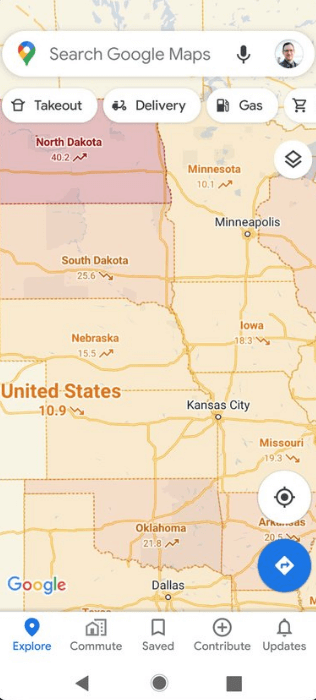
\includegraphics[width=0.45\linewidth,height=80mm]{state-level.png}
	}
	\subfigure[County Level]{
		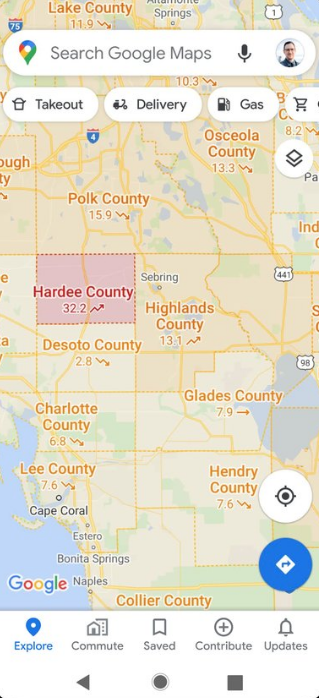
\includegraphics[width=0.45\linewidth,height=80mm]{county-level.png}
	}
	\caption{COVID layer in Google Map of different scales}
\end{figure}
\\
In Figure 6, \textbf{Google Map} adds a COVID-19 layer to the GIS, it also quantities an safety index by using the 7-day average for the number of new cases per 100,000 people.
It also indicates whether cases are increasing or decreasing.
The layer’s colors indicate:\footnote{https://support.google.com/maps/answer/9795160}
\begin{itemize}
	\item Grey: Less than 1 case
	\item Yellow: 1-10 cases
	\item Orange: 10-20 cases
	\item Dark orange: 20-30 cases
	\item Red: 30-40 cases
	\item Dark red: 40+ cases
\end{itemize}
Unlike \textbf{Google Map}, we perform the quantitative analysis based on dynamic GeoHash blocks instead of administrative regions.
The safety quantification algorithm we use not only includes the simple infected cases.
In the following chapters, I will focus on our research work about how to use GeoHash to improve the GIS in epidemic prevention and control.

\section{Pre-Work}
Our challenges are mainly from two aspects: data collection and data quantification.
Data collection is integrated in GIS, which requires user devices to upload their current positions, and the server needs to store the position data submitted by users.
Quantitative analysis of information is a more complex process and our work is to quantify collected data in GeoHash blocks.
\\
To the data collection, the system can provide a mobile application for users to view the surrounding epidemic situation.
At the same time, in order to obtain the surrounding epidemic safety situation, users need to upload their own GPS information.
Under the privacy policy, we only collect users' GPS information, but we will not save users' personal informationa. So we don't track or monitor users' positions.
This method of collection is carried out anonymously and each record is stored in the database as a virtual and unknown identity which means only users know their location but other users cannot get it.
After the diagnosis, health worker marks the infected case through the virtual user identity.
This means that the medical workers knows their patients' true identity, but even so, they cannot track their location information.
\\
To the data quantification, we need to divide the map to blocks first by using GeoHash.
At the step of GPS data collection, we get the longitude and latitude values from users, and we can use GeoHash to calculate which block the user belongs to.
Suppose a GeoHash block as a set \(B_1\) that includes many users, we quantify the safety of \(B_1\) based on confirmed cases and the total number of users in \(B_1\).
This is not enough, the historical ``visitors'' of this block also need to be considered too.
These visitors who are diagnosed in the short term will have negative effects on the block.
As we have discussed above (in Section 2.1), a research has proposed that the number of people infected in a region is positively correlated with the inflow of the population from high-risk areas.
That means, when collecting position data, we not only save a static current location, but also save a user's historical locations or blocks.
The general storage and calculation process is shown in Figure 7, and the detailed methods and algorithms are described in Section 4.
\begin{figure}[htb]
	\centering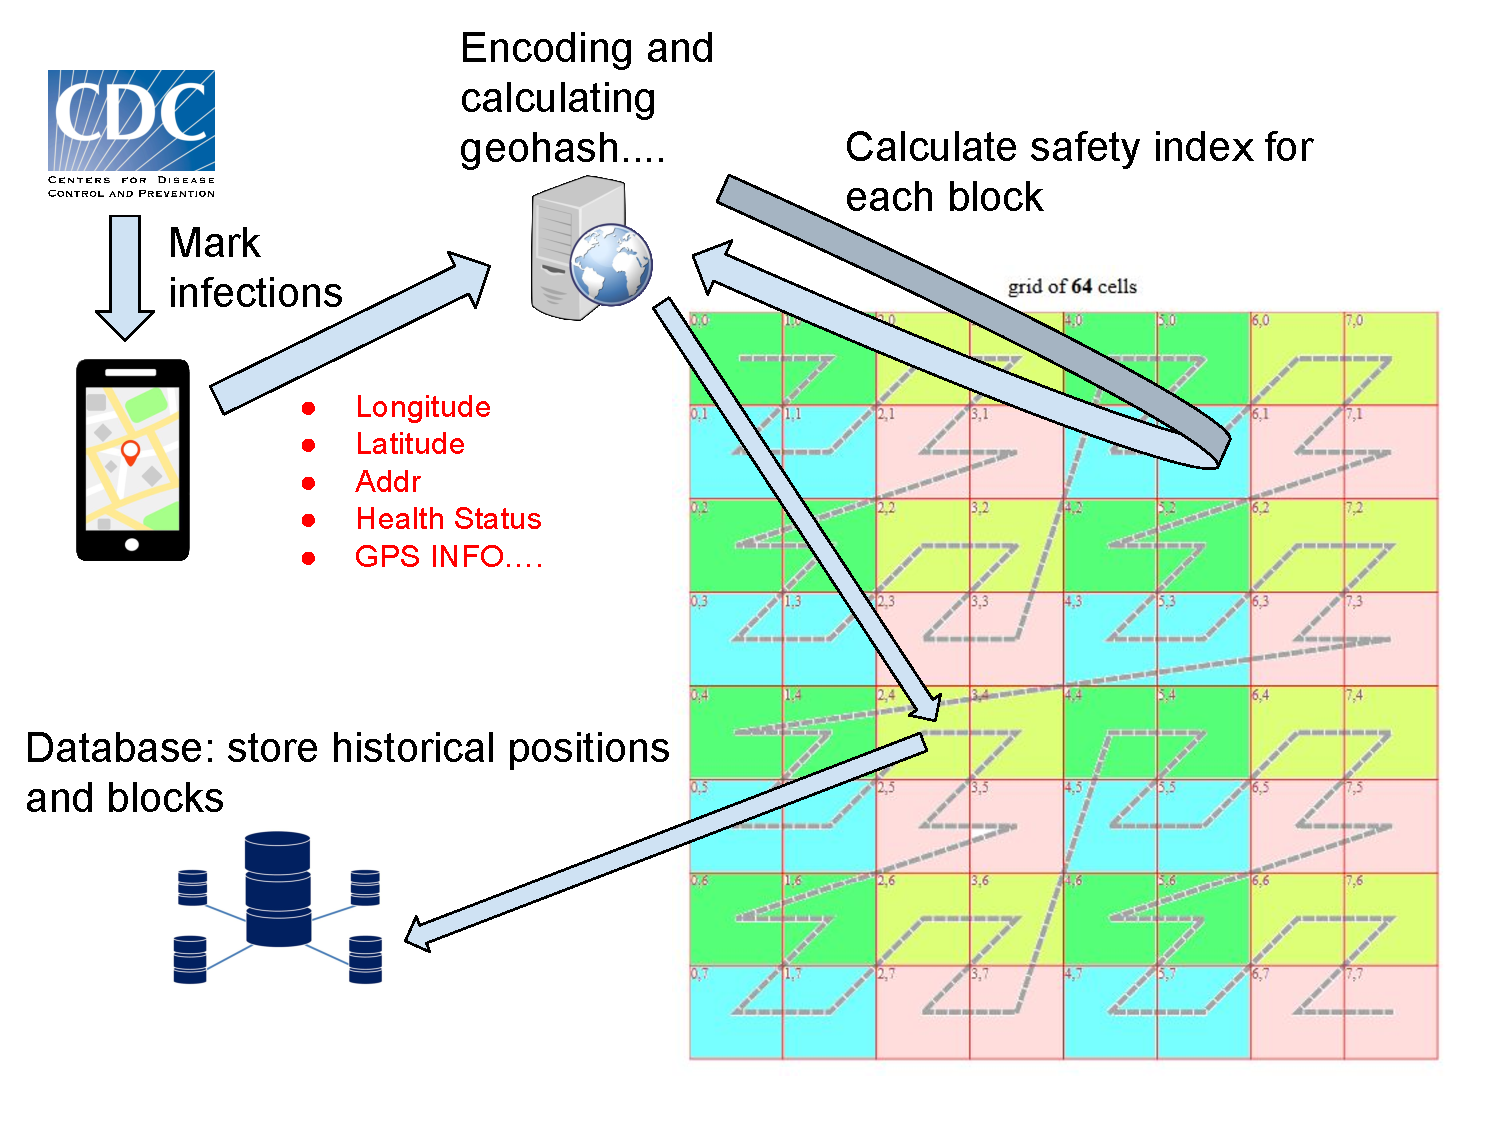
\includegraphics[width=\linewidth]{process.pdf}
	\caption{The process of data collection and quantification}
\end{figure}
\section{Algorithms and Methods}
\section{Test}
\section{Conclusions}
%%
%% The next two lines define the bibliography style to be used, and
%% the bibliography file.
\bibliographystyle{ACM-Reference-Format}
\bibliography{refs}
\end{document}
\endinput
